\documentclass{standalone}
\usepackage{tikz}
\usetikzlibrary{patterns, positioning}

\begin{document}
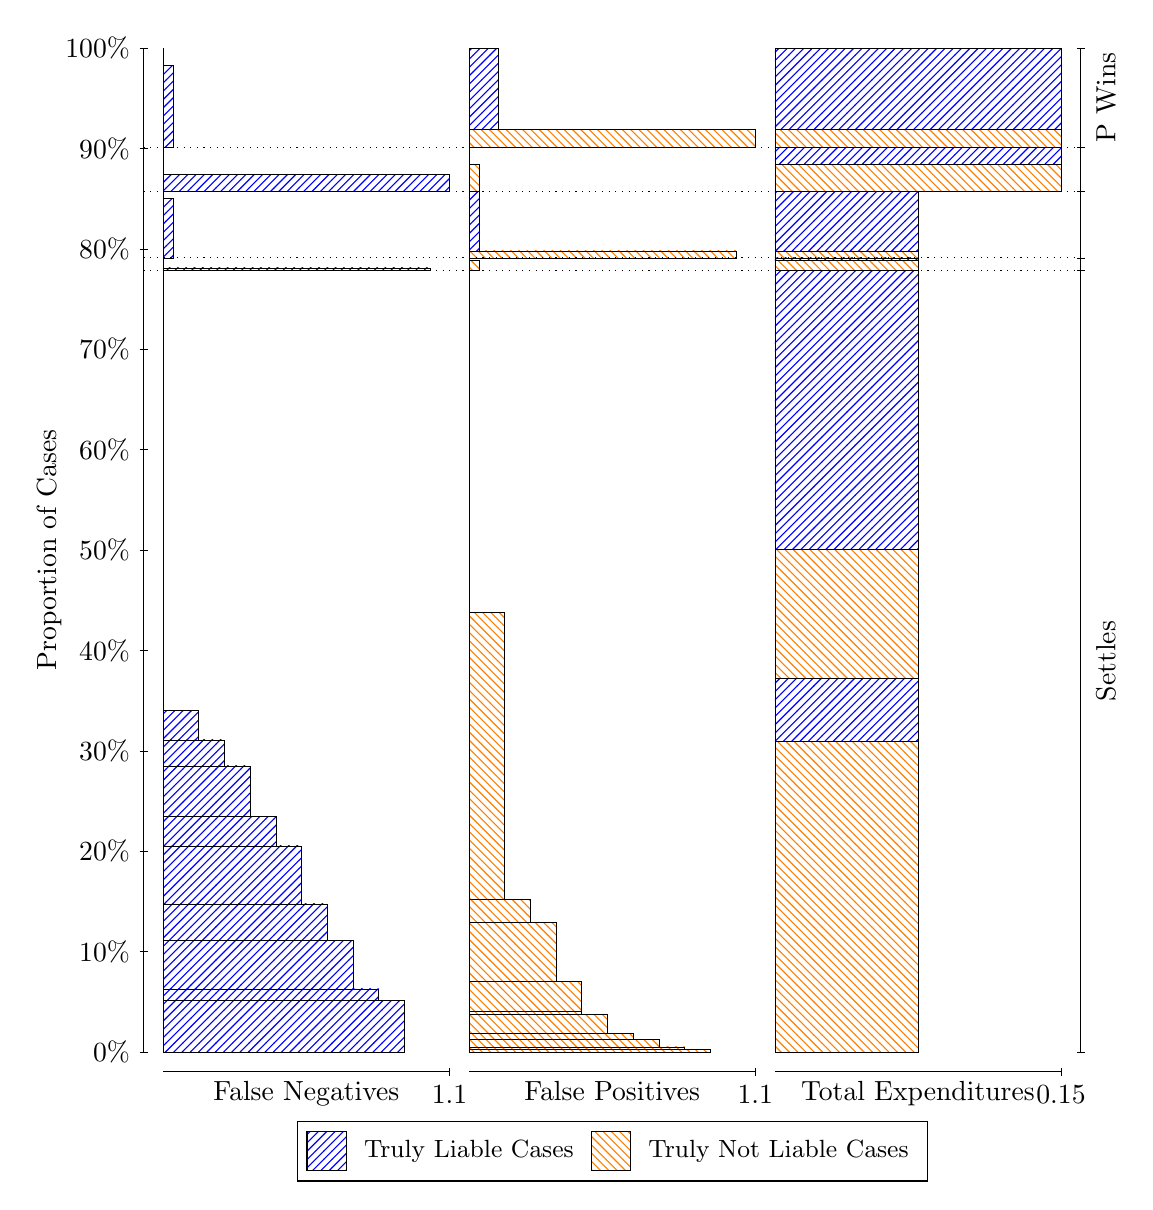
\begin{tikzpicture}
\draw[black, very thin] (1.5,1.75) -- (1.5,14.5);
\node[rotate=90, anchor=center] at (0.3, 8.125) {Proportion of Cases};
\draw[black, very thin] (1.45,1.75) -- (1.55,1.75);
\node[anchor=east] at (1.45, 1.75) {0\%};
\draw[black, very thin] (1.45,3.025) -- (1.55,3.025);
\node[anchor=east] at (1.45, 3.025) {10\%};
\draw[black, very thin] (1.45,4.3) -- (1.55,4.3);
\node[anchor=east] at (1.45, 4.3) {20\%};
\draw[black, very thin] (1.45,5.575) -- (1.55,5.575);
\node[anchor=east] at (1.45, 5.575) {30\%};
\draw[black, very thin] (1.45,6.85) -- (1.55,6.85);
\node[anchor=east] at (1.45, 6.85) {40\%};
\draw[black, very thin] (1.45,8.125) -- (1.55,8.125);
\node[anchor=east] at (1.45, 8.125) {50\%};
\draw[black, very thin] (1.45,9.4) -- (1.55,9.4);
\node[anchor=east] at (1.45, 9.4) {60\%};
\draw[black, very thin] (1.45,10.675) -- (1.55,10.675);
\node[anchor=east] at (1.45, 10.675) {70\%};
\draw[black, very thin] (1.45,11.95) -- (1.55,11.95);
\node[anchor=east] at (1.45, 11.95) {80\%};
\draw[black, very thin] (1.45,13.225) -- (1.55,13.225);
\node[anchor=east] at (1.45, 13.225) {90\%};
\draw[black, very thin] (1.45,14.5) -- (1.55,14.5);
\node[anchor=east] at (1.45, 14.5) {100\%};

\draw[black, very thin] (13.4,1.75) -- (13.4,14.5);
\draw[black, very thin] (13.35,1.75) -- (13.45,1.75);
\node[anchor=west] at (13.35, 1.75) {};
\draw[black, very thin] (13.35,11.678) -- (13.45,11.678);
\node[anchor=west] at (13.35, 11.678) {};
\draw[black, very thin] (13.35,11.835) -- (13.45,11.835);
\node[anchor=west] at (13.35, 11.835) {};
\draw[black, very thin] (13.35,12.675) -- (13.45,12.675);
\node[anchor=west] at (13.35, 12.675) {};
\draw[black, very thin] (13.35,13.242) -- (13.45,13.242);
\node[anchor=west] at (13.35, 13.242) {};
\draw[black, very thin] (13.35,14.5) -- (13.45,14.5);
\node[anchor=west] at (13.35, 14.5) {};

\draw[black, very thin, pattern color=blue, pattern=north east lines] (1.75,1.75) rectangle (4.8118,2.4069);
\draw[black, very thin, pattern color=blue, pattern=north east lines] (1.75,2.4069) rectangle (4.4852,2.5504);
\draw[black, very thin, pattern color=blue, pattern=north east lines] (1.75,2.5504) rectangle (4.1586,3.1668);
\draw[black, very thin, pattern color=blue, pattern=north east lines] (1.75,3.1668) rectangle (3.832,3.6295);
\draw[black, very thin, pattern color=blue, pattern=north east lines] (1.75,3.6295) rectangle (3.5054,4.3667);
\draw[black, very thin, pattern color=blue, pattern=north east lines] (1.75,4.3667) rectangle (3.1788,4.7447);
\draw[black, very thin, pattern color=blue, pattern=north east lines] (1.75,4.7447) rectangle (2.8522,5.3839);
\draw[black, very thin, pattern color=blue, pattern=north east lines] (1.75,5.3839) rectangle (2.5257,5.7141);
\draw[black, very thin, pattern color=blue, pattern=north east lines] (1.75,5.7141) rectangle (2.1991,6.0914);
\draw[black, very thin, pattern color=orange, pattern=north west lines] (1.75,6.0914) rectangle (1.75,11.678);
\draw[black, very thin, pattern color=blue, pattern=north east lines] (1.75,11.678) rectangle (5.1384,11.707);
\draw[black, very thin, pattern color=orange, pattern=north west lines] (1.75,11.707) rectangle (1.75,11.835);
\draw[black, very thin, pattern color=blue, pattern=north east lines] (1.75,11.835) rectangle (1.8725,12.586);
\draw[black, very thin, pattern color=orange, pattern=north west lines] (1.75,12.586) rectangle (1.75,12.675);
\draw[black, very thin, pattern color=blue, pattern=north east lines] (1.75,12.675) rectangle (5.3833,12.896);
\draw[black, very thin, pattern color=orange, pattern=north west lines] (1.75,12.896) rectangle (1.75,13.242);
\draw[black, very thin, pattern color=blue, pattern=north east lines] (1.75,13.242) rectangle (1.8725,14.276);
\draw[black, very thin, pattern color=orange, pattern=north west lines] (1.75,14.276) rectangle (1.75,14.5);
\draw[black, very thin, pattern color=orange, pattern=north west lines] (5.6333,1.75) rectangle (8.6951,1.7826);
\draw[black, very thin, pattern color=orange, pattern=north west lines] (5.6333,1.7826) rectangle (8.3685,1.816);
\draw[black, very thin, pattern color=orange, pattern=north west lines] (5.6333,1.816) rectangle (8.0419,1.9087);
\draw[black, very thin, pattern color=orange, pattern=north west lines] (5.6333,1.9087) rectangle (7.7154,1.988);
\draw[black, very thin, pattern color=orange, pattern=north west lines] (5.6333,1.988) rectangle (7.3888,2.2283);
\draw[black, very thin, pattern color=orange, pattern=north west lines] (5.6333,2.2283) rectangle (7.0622,2.2682);
\draw[black, very thin, pattern color=orange, pattern=north west lines] (5.6333,2.2682) rectangle (7.0622,2.6479);
\draw[black, very thin, pattern color=orange, pattern=north west lines] (5.6333,2.6479) rectangle (6.7356,3.3921);
\draw[black, very thin, pattern color=orange, pattern=north west lines] (5.6333,3.3921) rectangle (6.409,3.6918);
\draw[black, very thin, pattern color=orange, pattern=north west lines] (5.6333,3.6918) rectangle (6.0824,7.3371);
\draw[black, very thin, pattern color=blue, pattern=north east lines] (5.6333,7.3371) rectangle (5.6333,11.678);
\draw[black, very thin, pattern color=orange, pattern=north west lines] (5.6333,11.678) rectangle (5.7558,11.807);
\draw[black, very thin, pattern color=blue, pattern=north east lines] (5.6333,11.807) rectangle (5.6333,11.835);
\draw[black, very thin, pattern color=orange, pattern=north west lines] (5.6333,11.835) rectangle (9.0217,11.925);
\draw[black, very thin, pattern color=blue, pattern=north east lines] (5.6333,11.925) rectangle (5.7558,12.675);
\draw[black, very thin, pattern color=orange, pattern=north west lines] (5.6333,12.675) rectangle (5.7558,13.022);
\draw[black, very thin, pattern color=blue, pattern=north east lines] (5.6333,13.022) rectangle (5.6333,13.242);
\draw[black, very thin, pattern color=orange, pattern=north west lines] (5.6333,13.242) rectangle (9.2667,13.466);
\draw[black, very thin, pattern color=blue, pattern=north east lines] (5.6333,13.466) rectangle (6.0007,14.5);
\draw[black, very thin, pattern color=orange, pattern=north west lines] (9.5167,1.75) rectangle (11.333,5.695);
\draw[black, very thin, pattern color=blue, pattern=north east lines] (9.5167,5.695) rectangle (11.333,6.4954);
\draw[black, very thin, pattern color=orange, pattern=north west lines] (9.5167,6.4954) rectangle (11.333,8.1375);
\draw[black, very thin, pattern color=blue, pattern=north east lines] (9.5167,8.1375) rectangle (11.333,11.678);
\draw[black, very thin, pattern color=orange, pattern=north west lines] (9.5167,11.678) rectangle (11.333,11.807);
\draw[black, very thin, pattern color=blue, pattern=north east lines] (9.5167,11.807) rectangle (11.333,11.835);
\draw[black, very thin, pattern color=orange, pattern=north west lines] (9.5167,11.835) rectangle (11.333,11.925);
\draw[black, very thin, pattern color=blue, pattern=north east lines] (9.5167,11.925) rectangle (11.333,12.675);
\draw[black, very thin, pattern color=orange, pattern=north west lines] (9.5167,12.675) rectangle (13.15,13.022);
\draw[black, very thin, pattern color=blue, pattern=north east lines] (9.5167,13.022) rectangle (13.15,13.242);
\draw[black, very thin, pattern color=orange, pattern=north west lines] (9.5167,13.242) rectangle (13.15,13.466);
\draw[black, very thin, pattern color=blue, pattern=north east lines] (9.5167,13.466) rectangle (13.15,14.5);
\draw[black, dotted] (1.5,11.678) -- (13.4,11.678);
\draw[black, dotted] (1.5,11.835) -- (13.4,11.835);
\draw[black, dotted] (1.5,12.675) -- (13.4,12.675);
\draw[black, dotted] (1.5,13.242) -- (13.4,13.242);
\draw[black, very thin] (1.75,1.5) -- (5.3833,1.5);
\node[anchor=north] at (3.5667, 1.5) {False Negatives};
\draw[black, very thin] (5.3833,1.45) -- (5.3833,1.55);
\node[anchor=north] at (5.3833, 1.45) {1.1};

\draw[black, very thin] (5.6333,1.5) -- (9.2667,1.5);
\node[anchor=north] at (7.45, 1.5) {False Positives};
\draw[black, very thin] (9.2667,1.45) -- (9.2667,1.55);
\node[anchor=north] at (9.2667, 1.45) {1.1};

\draw[black, very thin] (9.5167,1.5) -- (13.15,1.5);
\node[anchor=north] at (11.333, 1.5) {Total Expenditures};
\draw[black, very thin] (13.15,1.45) -- (13.15,1.55);
\node[anchor=north] at (13.15, 1.45) {0.15};

\node[black, centered, rotate=90] at (13.72, 6.7142) {Settles};



\node[black, centered, rotate=90] at (13.72, 13.871) {P Wins};

\draw (7.449999999999999,1.5) node[draw=none] (baseCoordinate) {};
\begin{scope}[align=center]
        \matrix[scale=0.5, draw=black, below=0.5cm of baseCoordinate, nodes={draw}, column sep=0.1cm]{
            \node[rectangle, draw, minimum width=0.5cm, minimum height=0.5cm, pattern=north east lines, pattern color=blue] {}; &
            \node[draw=none, font=\small] (B) {Truly Liable Cases}; &
            \node[rectangle, draw, minimum width=0.5cm, minimum height=0.5cm, pattern=north west lines, pattern color=orange] {}; &
            \node[draw=none, font=\small] (B) {Truly Not Liable Cases}; \\
            };
\end{scope}

\end{tikzpicture}
\end{document}